\section{Electrodiffusion in the extracellular space}
\label{sec:Eldiff}
\index{Electrodiffusion}
By necessity, the transmembrane ionic currents produced by active neurons will cause the intra- and extracellular ion concentrations to change. Since neurons and glial cells contain numerous homeostatic mechanisms that work continuously to restore baseline concentrations, concentration changes are often limited to small deviances from baseline. For that reason, it is often a good approximation to assume that they remain constant, as one does when constructing multicompartment neurons as described in Chapter \ref{sec:Neuron}, and when using volume conductor (VC) theory as described in Chapter \ref{sec:VC}.

There are scenarios when the assumption of constant ion concentrations is not warranted. For example, during neuronal hyperactivity, or during several pathological conditions, the homeostatic machinery can fail to keep up, and ion concentrations may change rather dramatically, both in the intra- and extracellular space \citep{kraio1978, Dietzel1989, Somjen2001, Somjenboka, Frohlich2008, Zandt2015, Ayata2015}. Concentration changes will generally affect both (i) the transmembrane, (ii) the intracellular and (iii) the extracellular concentration gradients. If (i) transmembrane concentration gradients change, it will affect neuronal reversal potentials (cf. eq. \ref{Neuron:eq:revpots}), and this can have dramatic effects on neuronal firing properties (see e.g., \citep{Cressman2009, Zandt2011, Oyehaug2012, WeiUllahSchiff2014, Saetra2020}). If (ii) intracellular concentration gradients become large, longitudinal diffusion can dominate over electric drift currents, and standard multicompartment models, accounting only for the latter, 
become inaccurate \citep{Qian1989}. If (iii) extracellular concentration gradients become large, 
diffusive currents through the extracellular space can evoke so-called diffusion-potentials \citep{Gardner-Medwin1981, Dietzel1989, Halnes2016}. If present, these diffusion-potentials will give a contribution to the total extracellular potential ($\phi_e$), which are not accounted for
by standard VC-theory, where diffusive effects are assumed to be absent. 

We will start this Chapter by studying a simple example aimed to give an intuitive understanding of what a diffusion potential is and how it is generated through an electrodiffusive process (Section \ref{sec:Eldiff:LJpot}). Next, we will introduce the Nernst-Planck equation for electrodiffusive processes, and briefly introduce two alternative, physical framworks for solving it (Section \ref{sec:Eldiff:NP}). As we in this book focus on extracellular potentials, we are predominantly interested in the extracellular effects (iii) of ion concentration changes. We  will therefore present in some greater detail a framework for modeling extracellular electrodiffusion at the coarse-grained scale of tissue, and we will compare this framework to the standard VC-theory that we presented earlier (Section \ref{sec:Eldiff:porous}). Finally, we will use this framework to make some estimates of to which degree, and under which circumstances, diffusion potentials can be expected to be of non-negligible importance at the level of brain tissue (Section \ref{sec:Eldiff:estimates}).


\subsubsection{\blue{What is a diffusion potential?}}
\label{sec:Eldiff:LJpot}
\index{Diffusion potential}
Before doing any math, we may establish an intuitive understanding of the link between ion concentration dynamics and electric potentials by considering a simple two-compartment system with two ionic solutions interacting at a junction  (Fig. \ref{Eldiff:fig:diffpot}). Let us assume that the left compartment contains a high-concentration solution of NaCl, while the right compartment contains a low-concentration solution of NaCl (Fig. \ref{Eldiff:fig:diffpot}A). Let us further assume that both compartments are initially perfectly electroneutral, i.e.,the amounts of Na$^+$ and Cl$^-$ within each compartment are equal. No  electrical forces will then be present, and the initial system dynamics will be driven exclusively by diffusion. 

\begin{figure}[!ht]
\begin{center}
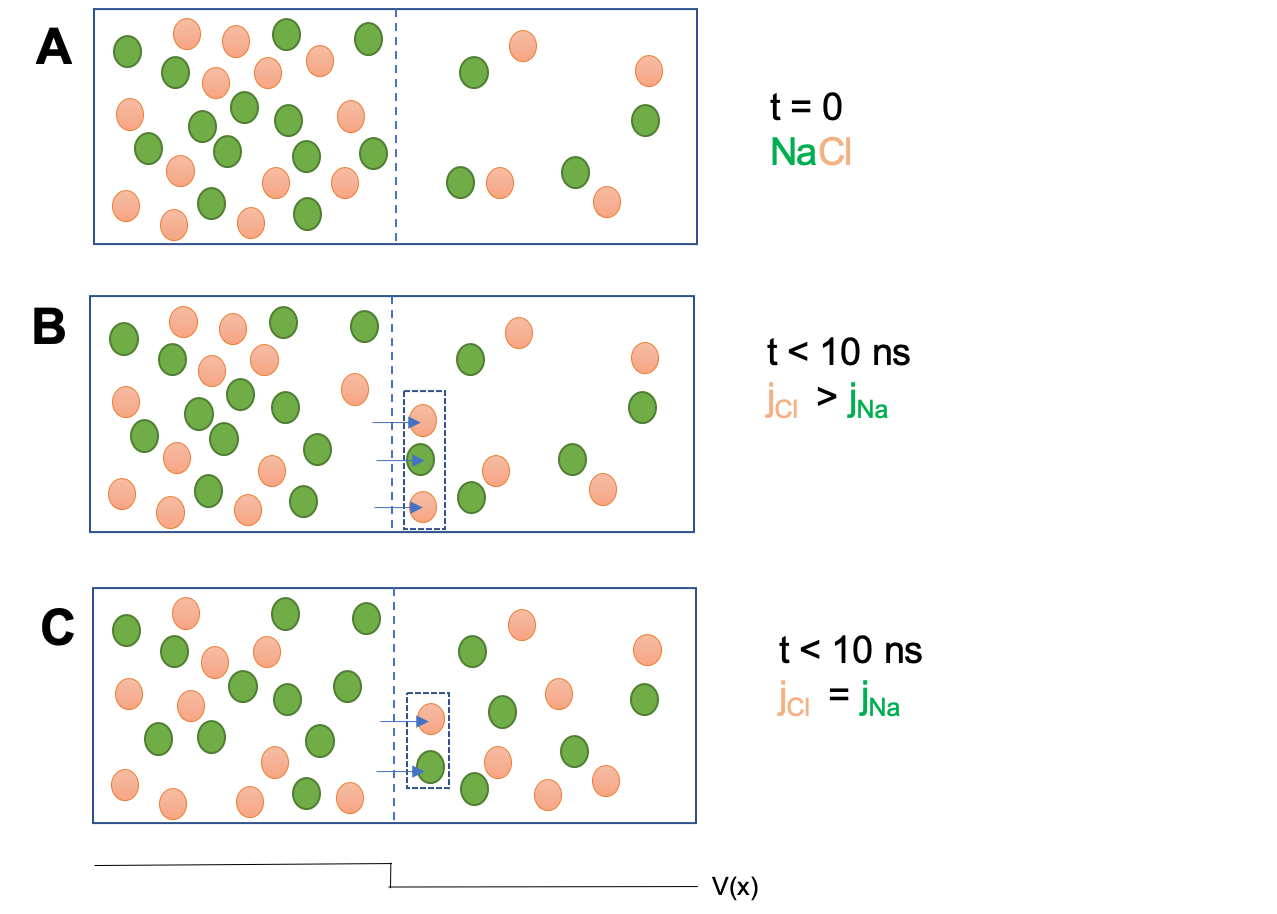
\includegraphics[width=0.8\textwidth]{Figures/Eldiff/Diffusionpot.png}
\end{center}
\caption{\textbf{Diffusion potential at the junction between two ionic solutions}. ({\bf A}) Initial condition with high concentration NaCl in the left compartment and low concentration NaCl in the right compartment. ({\bf B}) Since $D_{Cl} > D_{Na}$, we initially expect the flux of Cl$^-$ to be higher than the flux of Na$^+$. ({\bf C}) The net charge transfer in ({\bf B}) will give rise to a potential difference $\phi_d$ between the two compartments, which will prevent further charge accumulation. }
\label{Eldiff:fig:diffpot}
\end{figure}

We intuitively realize that both Na$^+$ and Cl$^-$ will diffuse towards the low-concentration compartment on the right-hand-side. Now, nature has it that not all ions diffuse equally fast, and the diffusive flux of a specific ion species will be proportional to its diffusion constant. From Table \ref{Sigma:tab:diffconsts}, we have that $D_{Na} = 1.33 \times 10^{-9}$ m$^2$/s, and $D_{Cl} = 2.03 \times 10^{-9}$ m$^2$/s in dilute solutions. Since $D_{Cl} > D_{Na}$, the rightward diffusive flux of Cl$^-$ will initially be larger than that for Na$^+$  (Fig. \ref{Eldiff:fig:diffpot}B). Diffusion thus acts as a charge separation process, resulting in an excess of positive charge in the left compartment and negative charge in the right compartment. The charge separation will in this way cause a potential difference ($\Delta \phi_d$) to arise between the compartments. Since $\Delta \phi_d$ stems from a diffusion process, it is often called the \textit{diffusion potential} \index{Diffusion potential}. Note that the diffusion potential arises due to differences in diffusion constants between different ions present. If all ions had identical diffusion constants, there would be no charge separation and thus no diffusion potential. 

The diffusion potential will oppose the on-going charge separation process by causing an electrical push on the anions (Cl$^-$) in the leftward direction, reducing the net rightward flux of Cl$^-$. Similarly, it causes a rightward pull on the cations (Na$^+$), increasing the net rightward flux of Na$^+$. Once it is gets big enough, $\Delta \phi_d$ will stabilize the system in a so-called quasi-steady state, where the net fluxes of Na$^+$ and Cl$^-$ have the same magnitude, and no further charge separation will take place (Fig. \ref{Eldiff:fig:diffpot}C). It has been shown that the extracellular medium of the brain only needs about 10 ns to reach this quasi-steady state \citep{Solbra2018}. In the quasi-steady state, $\Delta \phi_d$ will still vary with time (hence the term "quasi"), and eventually become zero when the system is equilibrated and the ion concentrations are the same in the two compartments. However, whereas the quasi-steady state is reached within a few nanoseconds, the concentration-equilibration process occurs at an entirely different time scale and normally takes seconds to minutes. 

Since it happens so fast, computer simulations of the charge separation process must be run with a sub-nanosecond time resolution. To simulate it is therefore computationally demanding, and not even feasible for large systems. Fortunately, one can for many purposes obtain accurate predictions of both $\Delta \phi_d$ and ion concentration dynamics by using an electroneutral mathematical framework that does not model the charge relaxation process explicitly, but instead derives an analytical expression for the quasi-steady state potential, and assumes that the system is always in quasi-steady state. We shall introduce the modeling frameworks for electrodiffusive processes later on in this Chapter. 

In electrolyte theory, the diffusion potential is often called the \textit{liquid-junction potential} \index{Liquid-junction potential}, since it is most pronounced at the junction between two different ionic solutions \citep{Aguilella1987, Sokalski2001}. Experimental neuroscientists should be acquainted with this term, since the determination of liquid-junction potentials is a common challenge when recording neural membrane potentials using patch clamp experiments. Through a process similar to that depicted in Fig. \ref{Eldiff:fig:diffpot}, only involving a larger number of different ion species, the liquid-junction potential develops at the junction between the pipette solution and the extracellular (or bath) solution, and give rise to a constant offset in the recordings, which must be estimated and corrected for \citep{barry1991,neher1992}. The magnitude of the liquid-junction potential depends on the composition of the various ion solutions, but in patch-clamp experiments it is typically a few millivolts. Other familiar examples of diffusion potentials in neuroscience are the ion channel reversal potentials (eq. \ref{Neuron:eq:revpots}), which are essentially single-ion diffusion potentials, and the leakage reversal potential (eq. \ref{Neuron:eq:Eleak_GHK}), which is a diffusion potential depending on the differences in passive membrane permeabilities (replacing the role of diffusion constants) of the various ion species. 

Compared to the reversal potentials and liquid-junction potentials in patch clamp experiments, 
diffusion potentials in the bulk solutions or the intra- or extracellular space tend to be smaller in magnitude, and have not been that much studied in neuroscience. Below, we will outline the general physical theory for determining the electric potential in electrodiffusive processes.


\subsection{The Nernst-Planck equation}
\label{sec:Eldiff:NP}
\index{Electrodiffusion}
When modeling an electrodiffusive process, we keep track of the ion concentration dynamics of each individual ion species. The fundamental equation for doing that is the Nernst-Planck equation for the flux density (${\bf j_k}$ of an ion species $k$:
\begin{equation}
{\bf j_k} = - D_k {\bf \nabla} c_{k} - \frac{D_k z_k c_k}{\psi} {\bf \nabla} \phi, 
\label{Eldiff:eq:eq:JNP}
\end{equation}
where ${D}_k$ is the diffusion constant (units $\mathrm{m^2/s}$), $z_{k}$ is the valency of ion species $k$, and $\psi=RT/F$ (units V) is defined by the gas constant ($R$), Faraday's constant ($F$) and the temperature ($T$). The first term on the right is Fick's law for diffusion, while the second term accounts for ions migrating in the electric field.  In eq. \ref{Eldiff:eq:JNP}, the the electrical mobility of the ions is $D_k/\psi$, and thus linearly related to their diffusion constant. This relationship is called the Einstein relation\index{Einstein relation}, and is valid for dilute solutions such as the extracellular or intracellular fluid \citep{Grodzinsky2011}.

If we combine eq. \ref{Eldiff:eq:JNP} with the requirement of ion conservation:
\begin{equation}
\frac{\partial c_k}{\partial t} = -\nabla \cdot {\bf j_k},
\label{Eldiff:eq:general_ionconservation}
\end{equation}
we get the Nernst-Planck continuity equation:
\begin{equation}
\frac{\partial c_k}{\partial t} = {\bf \nabla} \cdot \left[{D_k} {\bf \nabla} c_k + \frac{D_k z_k c_k}{\psi}{\bf \nabla} \phi \right].
\label{Eldiff:eq:NP}
\end{equation}

Eq. \ref{Eldiff:eq:NP} gives us one equation for each individual ion concentration $c_k$, and to solve the system of equations, we are in need an additional equation for the additional variable $\phi$, the electrical potential which couples the dynamics of the individual ion species. There are two main approaches to this, the so-called \textit{Poisson-Nernst-Planck (PNP)} framework, or the so-called \textit{electroneutral} framework, both of which we will introduce below. 


\subsubsection{\blue{The Poisson-Nernst-Planck (PNP) framework}}
\label{sec:Eldiff:PNP}
\index{Poisson-Nernst-Planck equations}
The physically most detailed approach for defining $\phi$ in eq. \ref{Eldiff:eq:NP}) is to use Poisson's equation from electrostatics:
\begin{equation}
\nabla^2 \phi = -\rho/\epsilon
\label{Eldiff:eq:poisson}
\end{equation}
Here $\epsilon$ is the (local) permittivity of the medium, and the local charge density $\rho$ can be expressed as a function of the ionic concentrations:
\begin{equation}
\rho = F\sum_k z_k c_k + \rho_0.
\label{Eldiff:eq:PNPrho}
\end{equation}
When we model ion concentrations, we normally do not include absolutely all ion species that are present, but rather chose to keep track of the most important ones (such as Na$^+$, K$^+$, Cl$^-$ and Ca$^{2+}$). For technical reasons, we therefore added a static charge density $\rho_0$\index{Static charge density} to eq \ref{Eldiff:eq:PNPrho}, which to accounts for all charges not included in the set $c_k$. 

Combined with suitable boundary conditions, the PNP equations (eq. \ref{Eldiff:eq:NP} together with eq. \ref{Eldiff:eq:poisson}) can in principle be solved for arbitrary complex geometries using numerical methods, like the Finite Element Method (FEM). 


\subsubsection{\blue{The electroneutral framework}}
\label{sec:Eldiff:electroneutral}
\index{Electroneutral}
An alternative to the PNP approach is to replace the Poisson equation (eq. \ref{Eldiff:eq:poisson}) with the approximation that the bulk solution is electroneutral:
\begin{equation}
F \sum_k z_k c_k + \rho_0 = 0.
\label{Eldiff:eq:electroneutral}
\end{equation}
In practice, it is often more convenient to impose the electroneutrality approximation on differential form:
\begin{equation}
F \sum_k{z_k \frac{\partial c_k}{\partial t}} = 0.
\label{Eldiff:eq:electroneutral2}
\end{equation}

The electroneutrality approximation (eq. \ref{Eldiff:eq:electroneutral} or \ref{Eldiff:eq:electroneutral2}) can be imposed as a constraint when solving eq.\ref{Eldiff:eq:NP} by use of some numerical method. The constraint determines what $\phi$ must be at all points in space for there to be no charge accumulation anywhere in the extracellular or intracellular bulk solutions. As soon as reference point (i.e., ground, $\phi = 0$) is set, this problem has a unique solution.


\subsubsection{\blue{The difference between the PNP and electroneutral frameworks}}
\label{sec:Eldiff:CompareFrameworks}
To explain how the electroneutral framework differs from the PNP framework, we may use our previous cartoon example (Fig. \ref{Eldiff:fig:diffpot}) as a reference. As we there explained, the diffusion potential is (i) evoked by charge separation process that only lasts for $\sim 10$ ns, and is (ii) most pronounced at the junction between two solutions of different ionic composition. In neural tissue, nonzero charge densities are predominantly resolved in nano-meter thick layers around neuronal membranes \citep{Grodzinsky2011, Gratiy2017}. 

The PNP framework explicitly models the nanosecond-fast charge relaxation processes (Fig. \ref{Eldiff:fig:diffpot}B), and must ensure that the ionic concentrations at all points sum up to the correct charge density (cf. eq. \ref{Eldiff:eq:PNPrho}). Since the deviance from electronutrality associated with $\rho$ involves a only very tiny fraction of the ions present \citep{Aguilella1987}, stable PNP simulations require that $c_k$ is determined with an extreme precision. PNP simulations therefore require a spatiotemporal resolution smaller than nanometers and nanoseconds, and thus a very fine-grained description of the tissue where neuronal, glial and extracellular geometries are explicitly defined. This makes PNP simulations extremely computationally demanding, and not suited for estimating dynamics at the level of tissue. Applications in neuroscience have therefore been limited to studies of electrodiffusive processes taking place on a very tiny spatiotemporal scale, such as in dendritic spines or near and inside membranes (see e.g., \citep{Leonetti2004, Lu2007, Lopreore2008, Nanninga2008, Gardner2011, Zheng2011, Pods2013, Gardner2015, lagache2019, cartailler2019}). See \citep{Savtchenko2017} for a review of applications in neuroscience.

In contrast, the electroneutral framework circumvents the charge relaxation problem by assuming (and ensuring) that the system is always in quasi-steady (Fig. \ref{Eldiff:fig:diffpot}C), and uses the electroneutrality constraint (eq. \ref{Eldiff:eq:electroneutral} or \ref{Eldiff:eq:electroneutral2}) to derive the potential $\phi$ required for this to be the case. 
Although electroneutrality at a fundamental level is inconsistent with a non-zero $\phi$ (cf. eq. \ref{Eldiff:eq:poisson}), the electroneutral approach still give accurate predictions of both $c_k$ and $\phi$ under many circumstances \citep{Feldberg2000}, since the fraction of ions associated with the deviance from electroeutrality is so small. In biophysical applications, it has been shown that the electroneutral approximation gives accurate results on spatiotemporal scales larger than micrometers and microseconds \citep{Grodzinsky2011, Pods2017, Solbra2018}. The advantage with the electroneutral approach is that it, unlike PNP, gives stable solutions with an arbitrary coarse spatiotemporal resolution, making the electroneutral framework much more computationally efficient than the PNP framework . 

Both the PNP and electroneutral framework require numerical solutions based on finite element or finite difference methods. While the electroneutral framework is computationally much more efficient than the PNP framework, it is still too heavy to allow for simulations of large systems of neurons described with explicit geometries on today's computers. To our knowledge, the largest system that so far has been simulated in 3D on an electroneutral framework is small piece of tissue containing a bundle of 9 axons described with idealized geometries \citep{ellingsrud2020}.


\subsubsection{\blue{Membrane boundary conditions}}
\label{sec:Eldiff:BCs}
To apply one of the electrodiffusive frameworks within a neuroscience context, one needs to represent the geometry and properties of the cellular membranes. In principle, we could compute all ionic concentrations and their coupling to the electrical potential by requesting that eq. \ref{Eldiff:eq:NP} should be fulfilled at all points in space, including both the extracellular space, the intracellular space and the membranes separating them. This could be achieved through having spatially and temporally varying diffusion coefficients $D_k$. However, the resolution with which one needed to represent $D_k$ would then be extremely high. Whereas $D_k$ could have a constant value in the intra- and extracellular bulk solutions, $D_k$ would over the membranes be (i) different in different spatial directions (i.e., normal to membrane surface versus parallel to membrane surface), (ii) vary with the very fine spatial resolution of an ion channel, and (iii) also be time dependent due to the opening/closing of ion channels. Unless the PNP scheme is applied to specifically model currents inside ion channels on a very small spatial scale (see e.g., \citep{Gardner2011, Zheng2011}), such a fine-grained tensor description of $D_k$ does not seem like a reasonable approach. 

Instead, it is common to rather apply the PNP or electroneutral framework in two disjoint domains - the intra and extracellular - and to couple the dynamics in these two domains by introducing suitable boundary conditions at the membrane. In many applications, the membrane dynamics is then based on a Hodgkin-Huxley (HH) type formalism (c.f., Section \ref{sec:Neuron:membranecurrents}) also in PNP based (see e.g., \citep{Lopreore2008, Pods2013, Gardner2015, Pods2017}) or electroneutral (see e.g., \citep{Mori2006, Mori2009, Pods2017, ellingsrud2020}) models. When applying a HH formalism in this context, all transmembrane currents are made ion specific, i.e., they are described in terms of ionic fluxes over the membrane, so that for example a Na$^+$ current density ($i_{Na}$) in the standard HH formalism would need to be replaced with a Na$^+$ flux density, $j_{Na} = i_{Na}/(Fz_k)$. The leakage current ($i_L$ in eq. \ref{Neuron:eq:HHleak}) is in standard HH applications non-specific in terms of which ions that mediate it, but will in a PNP context have to be made ion specific by decomposing it into specific leakage fluxes of the various ions that are involved (see e.g., \citep{Pods2013}). Apart from that, the HH formalism for membrane mechanisms can be applied in its original form also in an electrodiffusive context.

We note that in electroneutral frameworks, the electroneutrality constraint (eq. \ref{Eldiff:eq:electroneutral} or \ref{Eldiff:eq:electroneutral2}) applies only to the intra- and extracellular bulk solutions, and must be replaced with another constraint at the membrane, where a non-zero membrane (surface) charge density ($\eta^{mem}$ (C/m$^2$)) builds up the membrane potential according to the capacitor relationship:
\begin{equation}
c_m \phi_{m} = \pm \eta_{r}^{mem},
\label{Eldiff:eq:rhocap}
\end{equation}
or its temporal derivative: 
\begin{equation}
i_{cap} = \pm \frac{\partial \eta_{r}^{mem}}{\partial t},
\label{Eldiff:eq:rhocapt}
\end{equation}
Here, $c_m$ (F/m$^2$) in eq. \ref{Eldiff:eq:rhocap} is the specific membrane capacitance, and the left hand side of eq. \ref{Eldiff:eq:rhocapt} follows the definition is the capacitive membrane current density $i_{cap}$  (eq. \ref{Neuron:eq:HHcap}). In both equations, $r$ takes the indices $i$ (intracellular side of the membrane) or $e$ (extracellular side of the membrane), and the plus-sign should be used for $r=i$, and the minus-sign for $r=e$, a convention that follows from the definition $\phi_{m} = \phi_{i} - \phi_{e}$. The intra- and extracellular membrane charge densities in eq. \ref{Eldiff:eq:rhocap} or their derivatives in \ref{Eldiff:eq:rhocapt} are equal in magnitude and opposite in sign, since the charge stored on one side of a capacitor always balances the charge stored on the other side. 

For the electroneutrality constraint at the membrane (eq. \ref{Eldiff:eq:rhocap} or \ref{Eldiff:eq:rhocapt}) to be useful, $\eta_{r}^{mem}$ must be expressed in terms of the ion concentrations. That is, one needs an additional condition to specify the composition of ions that constitute $\eta_{r}^{mem}$ in eq. \ref{Eldiff:eq:rhocap} or mediate $i_{cap}$ in eq. \ref{Eldiff:eq:rhocapt}, so that ion conservation and a consistent charge-concentration relationship  at all points in space is ensured. Previous schemes for implementing the electroneutral framework vary somewhat in the approach taken to this:

\begin{itemize}
\item The electroneutral scheme with internal boundary conditions at membranes (ENM), derived the concentration profile of the membrane charge density $\eta_{r}^{mem}$ from a set of constraints as to how ion concentrations are distributed within the Debye-layer \citep{Mori2006, Mori2009, Pods2017}.

\item The Kirchhoff-Nernst-Planck (KNP) scheme did not resolve Debye-layer concentrations, but let the membrane concentration profile follow from an assumption regarding how much various ion species contributed to the capacitive membrane current $i_{cap}$ \citep{ellingsrud2020}.
\end{itemize}

Both electroneutral schemes (ENM and KNP) were designed so that the membrane concentration profiles were functions of, and similar to, the concentration profiles in the bulk solution close to the membrane. Although they differ in implementation details, the two schemes should be close to equivalent from a physics point of view, except at Debye layer-resolution close to the membrane.  In practice, only a very tiny fraction of the ions present are involved in building up the membrane potential, and the choice as to which ion species that actually constitute the membrane charge in eq. \ref{Eldiff:eq:rhocap} or \ref{Eldiff:eq:rhocapt} is probably quite unimportant for the overall system dynamics.


\subsection{\blue{Extracellular electrodiffusion in brain tissue}}
\label{sec:Eldiff:porous}
\index{sec:Eldiff:Tissue}
From here on, we will consider electrodiffusion at the scale of tissue, and we shall treat the tissue as a continuous porous medium. This is similar to how we treated the tissue as a continuous volume conductor in Chapter \ref{sec:VC}, the difference being that we now, in addition to keeping track of the extracellular potential ($\phi$), will be keeping track also of the extracellular concentrations ($c_k$) of all mobile ion species within the medium. 

In standard applications of VC theory, the neurodynamics is computed in an independent step (Step 1) under the assumption that it is independent of whatever goes on in the extracellular space. The transmembrane neuronal currents are then, in a next step (Step 2), considered as distributed current sources and sinks within the tissue. A similar approach can been taken to study extracellular electrodiffusion, e.g., by combining HHC-type neuron models (Step 1) with an electroneutral electrodiffusive framework (Step 2) such as the so-called Kirchhoff-Nernst-Planck (KNP) framework presented in \cite{Solbra2018}. The procedure is then:

\begin{itemize}
\item {\bf Step 1:} Compute neurodynamics using a standard HHC-type framework (Chapter \ref{sec:Neuron}). Unlike in the standard HHC+VC scheme, where the different kinds of transmembrane currents, such as leakage currents, capacitive currents, and ion specific active currents, can be grouped into a single source variable $C$ for the total current source density (CSD) at each segment, an electrodiffusive treatment requires that all neural sources are expressed as a set of ion specific sources, i.e., one source $f_k$ per ion species $k$ and an additional capacitive neuronal membrane current source density, $C_e^{cap}$ (proportional to $i_{cap}$ in eq. \ref{Eldiff:eq:rhocapt}), the only source term not accounted for in the set $f_k$. These variables, along with other relevant variables, will be defined properly below (Section \ref{sec:Eldiff:porous}).

\item {\bf Step 2:} Use an electrodiffusive framework to compute the dynamics of $c_k$ and $\phi$ in the extracellular space when "receiving" input from discrete neuronal sources computed in Step 1 (Fig. \ref{Eldiff:fig:KNPmesh}). The Nernst-Planck continuity equation (eq. \ref{Eldiff:eq:NP}) is then applied exclusively to the extracellular space, and the neural output is expressed through the source terms ($f_k$ and  $C_e^{cap}$). In the following, we will present the KNP framework for extracellular electrodiffusion within this two-step scheme.
\end{itemize}

\begin{figure}[!ht]
\begin{center}
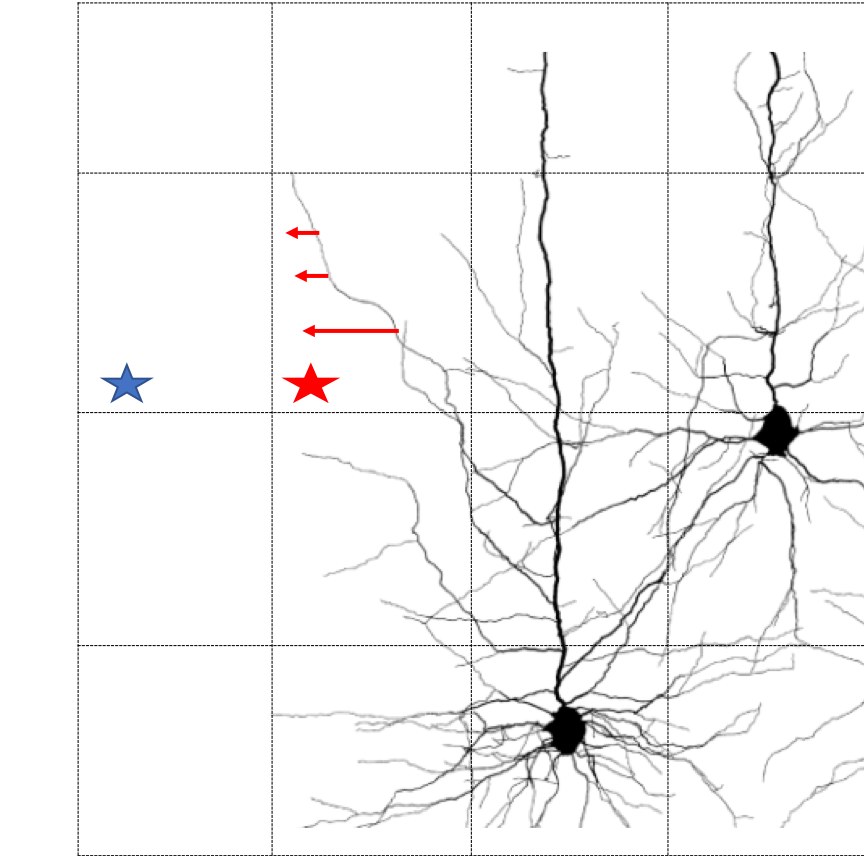
\includegraphics[width=0.5\textwidth]{Figures/Eldiff/KNP.png}
\end{center}
\caption{\textbf{KNP scheme}. Blue star: Mesh cell containing no neuronal sources, so that $C=0$. Red star: Mesh cell containing neural sources. Here $C$ can be computed by summing over all neuronal transmembrane currents, including the capacitive current, and dividing by the volume of the mesh cell. \ghnote{LAGE LITT MER INFORMATIV FIG HER OM VI SKAL HA FIG HER.}}
\label{Eldiff:fig:KNPmesh}
\end{figure}


\subsubsection{\blue{Continuous, porous medium approximation for electrodiffusion in tissue}}
\label{sec:Eldiff:porous}
\index{Continuous medium}
\index{Porous medium}
In Section \ref{sec:Sigma:continuous}, we introduced the continuous, porous medium approximation for coarse grained volume conduction in brain tissue, and we will use a similar approximation for electrodiffusive processes through the tissue. As in Section \ref{sec:Sigma:continuous}, 
the key parameters for defining the porous medium are the extracellular volume fraction $\alpha$ and the tortuosity, $\lambda$ (Fig. \ref{Eldiff:fig:porous}). However, unlike what we did in Section \ref{sec:Sigma:continuous}, where our reference volume was the tissue as a whole, we shall here follow the convention that we use as reference volume only the fraction $\alpha$ of tissue that is extracellular space \citep{Sykova2008}. As we shall see, this convention offers the most natural definition of the extracellular concentrations. 

\begin{figure}[!ht]
\begin{center}
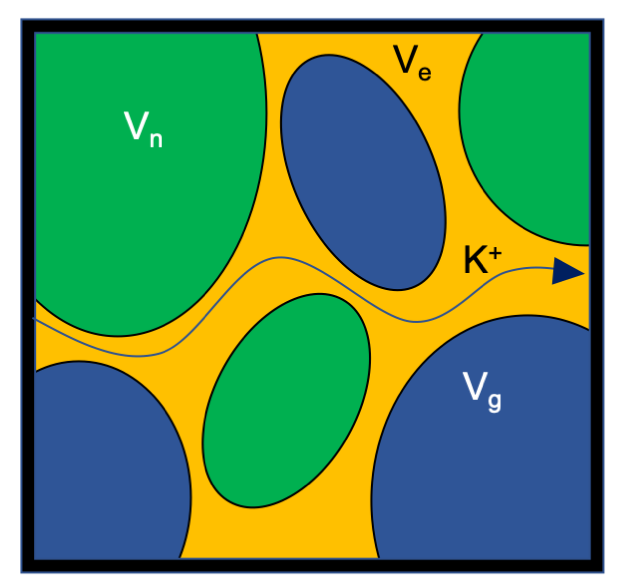
\includegraphics[width=0.5\textwidth]{Figures/Eldiff/Porous.png}
\end{center}
\caption{\textbf{Tortuous, porous medium.}  Sketch of a cross-section of a piece of neural tissue. Extracellular space (yellow) occupies a fraction $\alpha$ (about 0.2 of the total tissue volume), while neurons and glial cells occupy about equally much of the remaining space. The extracellular space has a highly tortuous structure. We consider tissue transport processes that are confined to occur only in the extracellular part of the tissue. Detours around neuronal and glial obstacles are accounted for by the tortuosity $\lambda$. 
\tvnnote{kanskje med panel B en zoomet ut versjon der det ser mer homogent ut? Hadde Klas allerede laget en lignende figur til Sterratt? }
}
\label{Eldiff:fig:porous}
\end{figure}

If we define all extracellular variables relative to the extracellular volume fraction  (Fig. \ref{Eldiff:fig:porous}), they can be defined as:

\begin{itemize}
\item $c_k$ (units $\mathrm{mol/m^3}$ = mM) is the extracellular concentration of an ion species $k$, defined as the number of extracellular ions of species $k$ (in mol) per extracellular volume unit (which is a fraction $\alpha$ of the tissue volume unit). The motivation for using the extracellular volume fraction as the reference volume is that concentrations defined in this way will be the "real" extracellular concentration, i.e., the concentration experienced by a neural membrane, 

\item $\rho_e$ (units $\mathrm{C/m^3}$) is the extracellular charge density
of an ion species $k$, defined as the number of extracellular ions of species $k$ (in mol) per extracellular volume unit (which is a fraction $\alpha$ of the tissue volume unit).

\item ${\bf j_k}$ (units $mol/\mathrm{m^2s}$) is the extracellular flux density of an ion species $k$, defined as the number of extracellular ions (in mols) crossing an extracellular unit cross- section area (which is a fraction $\alpha$ of a unit tissue cross-section area) per second.

\item  ${\bf i_e}$ (units $\mathrm{A/m^2}$) is the extracellular current density, defined as extracellular current per per extracellular unit cross-section area. In comparison, the current density ${\bf i}$ in Chapter \ref{sec:VC} was defined as extracellular current per unit tissue cross-section area, which means that ${\bf i_e} = {\bf i}/\alpha$.

\item $\tilde{D}_k$ (units $\mathrm{m^2/s}$) is the effective diffusion constant \index{Diffusion constant} for ion species $k$ in the extracellular medium. It is defined so that the diffusive flux is given by ${\bf j_k^{diff}} = -\tilde{D}_k \nabla c_k$ \citep{nicholson2001}. The effective diffusion constant accounts for the fact that diffusing ions face obstacles (neurites) along their path forcing them take detours, reflected through a tortuosity $\lambda$ which has a value of about 
$1.6$ in the extracellular space \citep{Nicholson1998}. The effective diffusion constant is given by:
\begin{equation}
\tilde{D_k} = \frac{D_k}{\lambda^2}, 
\label{Eldiff:eq:diffconst}
\end{equation}
where $D_k$ is the diffusion constant for an ion species $k$ in the pure (unhindered) extracellular solution. The fact that diffusing ions are confined the stay only in the extracellular volume fraction $\alpha$ is already accounted for in the flux definition. 

\item $\sigma_e$ (units S/m) is the tissue averaged extracellular conductivity for extracellular current densities defined as ${\bf i_e}$. As we show later, $\sigma_e$ can be expressed as a function of ion concentrations:
\begin{equation}
\sigma_e = \frac{F}{\psi}\sum_{k} \tilde{D}_k z_{k}^2 c_{k}.
\label{Eldiff:eq:sigma1}
\end{equation}
Here $z_{k}$ is the valency of ion species $k$, and $\psi=RT/F$ is defined by the gas constant ($R$), Faraday's constant ($F$) and the temperature ($T$). Since $\sigma_e$ relates to ${\bf i_e}$ in the same way that the tissue conductivity, $\sigma_t$, related to ${\bf i_t}$ in Chapter \ref{sec:VC}, $\sigma_e = \sigma /\alpha$.

\item $f_k$ (units mol/m$^3$) is the ion-flux-source density, i.e., the local neuronal output of an ion species $k$ per per extracellular volume unit. It is essentially is the ion-dynamics counterpart to the current-source-density (CSD) presented earlier (eq. \ref{VC:eq:CSD1}).

\item $C_e$ (units A/m$^3$) is the current source density, i.e., the local neuronal output current per extracellular volume unit. $C_e = C/\alpha$ where $C$ (as defined in Chapter \ref{sec:VC}) is neuronal output current per tissue volume unit.
\end{itemize}


\subsubsection{\blue{Dynamics of ion concentrations}}
\label{sec:Eldiff:ionconcentrationdynamics}
In the coarse-grained description, using the effective diffusion constant, $\tilde{D}_k$, the flux density (${\bf j_k}$) of an ion species $k$ is given by:
\begin{equation}
{\bf j_k} = - \tilde{D}_k {\bf \nabla} c_{k} - \frac{\tilde{D}_k z_k c_k}{\psi} {\bf \nabla} \phi.
\label{Eldiff:eq:JNP}
\end{equation}
The first term on the right hand side of eq. \ref{Eldiff:eq:JNP} is the ionic flux density due to diffusion (${\bf j_{k}^\text{diff}}$), and the second term is the additional flux density due to electrical drift along gradients in the extracellular potential $\phi$ (${\bf j_{k}^\text{drift}}$). 

The general continuity equation for an ion species $k$ is,
\begin{equation}
\frac{\partial c_k}{\partial t} = - \nabla \cdot {\bf j_k} + f_k,
\label{Eldiff:eq:salamander}
\end{equation}
where we have included the neuronal source term $f_k$. If we insert the electroduffusive flux density (eq. \ref{Eldiff:eq:JNP}) into eq. \ref{Eldiff:eq:salamander}, we get the Nernst-Planck continuity equation:
\begin{equation}
\frac{\partial c_k}{\partial t} = {\bf \nabla} \cdot \left[ \tilde{D}_k {\bf \nabla} c_k + \frac{\tilde{D}_k z_k c_k}{\psi} {\bf \nabla} \phi \right] + f_k.
\label{Eldiff:eq:NP}
\end{equation}
This equation is the fundamental equation in the KNP scheme. Eq. \ref{Eldiff:eq:NP} gives us one equation for each individual ion concentration $c_k$, and to solve the system of equations, we are in need an additional equation for the additional variable $\phi$. 


\subsubsection{\blue{Dynamics of the extracellular potential}}
\label{sec:Eldiff:electrodynamics}
From the equations for ion concentration dynamics (eqns. \ref{Eldiff:eq:JNP}-\ref{Eldiff:eq:NP} ) we can derive a corresponding set of equations for net charge dynamics. This will also allow us to derive the expression for $\phi$ that we need in order to solve the Nernst-Planck equation (eq. \ref{Eldiff:eq:NP}).  It will also show us how they relate to to the VC theory presented in Chapter \ref{sec:VC}.

If we multiply eq. \ref{Eldiff:eq:JNP} by $F\cdot z_k$ and sum over all ion species $k$, we get the extracellular current density:
\begin{equation}
{\bf i_e} = F\sum_k {z_k {\bf j_k}} = -\sum_k{F z_k \tilde{D_k}{\bf \nabla} c_{k}} - F\sum_{k} \frac{\tilde{D_k} z_{k}^2}{\psi}c_{k} {\bf \nabla}{\phi}, 
\label{Eldiff:eq:INPa}
\end{equation}
where the first term on the right hand side is the diffusive current density ${\bf i_e^\text{diff}}$, and the second term is the Ohmic drift current density ${\bf i_e^\text{drift}}$. Since we know from earlier that the drift current density should equal $- \sigma_e \nabla \phi$  (cf. eq. \ref{VC:eq:ohmici}) we may identify the the conductivity $\sigma_e$ of the extracellular medium as \citep{Koch1999}:
\begin{equation}
\sigma_e = \frac{F}{\psi}\sum_{k} \tilde{D}_k z_{k}^2 c_{k},
\label{Eldiff:eq:sigma}
\end{equation}
as we postulated in eq. \ref{Eldiff:eq:sigma1}. With this, we can write eq. \ref{Eldiff:eq:INPa} on the simpler form:
\begin{equation}
{\bf i_e} = - \sum_k{F z_k \tilde{D_k}{\bf \nabla} c_{k}} - \sigma_e{\bf \nabla}{\phi},
\label{Eldiff:eq:INP}
\end{equation}

Likewise, if we multiply eq. \ref{Eldiff:eq:salamander} by $F\cdot z_k$ and sum over all ion species, we get the continuity equation for charge: 
\begin{equation}
\frac{\partial \rho_e}{\partial t} =  \nabla \cdot \left (\sum_k{F z_k \tilde{D_k}{\bf \nabla} c_{k}} + \sigma_e\nabla\phi  \right)  + C_e^{ion}.
\label{Eldiff:eq:chargecontinuity}
\end{equation}
We have here introduced the extracellular charge density (define as extracellular charge per tissue unit volume), 
\begin{equation}
\rho_e = F \sum_k z_k c_k + \rho_{0e},  
\label{Eldiff:eq:roen}
\end{equation}
and the ionic current source, 
\begin{equation}
C_e^{ion} = F \sum_k z_k f_k. 
\label{Eldiff:eq:csden}
\end{equation}
The term $\rho_{0e}$ in eq. \ref{Eldiff:eq:roen} represents a static extracellular charge density representing charged macromolecules and any species' of ions that are not included in the set $c_k$, and which is assumed to be constant in time and space. The index "ion" in eq. \ref{Eldiff:eq:csden} signifies that this source term exclusively accounts for the sources $f_k$ mediated by ions that pass through the neuronal membrane and enters or leaves the extracellular space in eq. \ref{Eldiff:eq:NP}. Importantly, $C_e^{ion}$ is not identical to the total CSD, which contains an additional capacitive component that accounts for the accumulation of a charge density $\rho_e^{mem}$ (defined as membrane charge per extracellular unit volume) at the exterior side of the neuronal membrane:
\begin{equation}
C_e = C_e^{ion} + C_e^{cap} = F \sum_k z_k f_k - \frac{\partial \rho_{e}^{mem}}{\partial t}.
\label{Eldiff:eq:CSDdecomposed}
\end{equation}
$C_e^{cap}$ interprets as the neuronal capacitive membrane current per extracellular unit volume (see Fig. \ref{Eldiff:fig:Ccap}), and the negative sign in front of the last term in \ref{Eldiff:eq:CSDdecomposed} follows from the fact that an outwards capacitive current (i.e., a source) implies an accumulation negative charge on the exterior side of the membrane. 

\begin{figure}[!ht]
\begin{center}
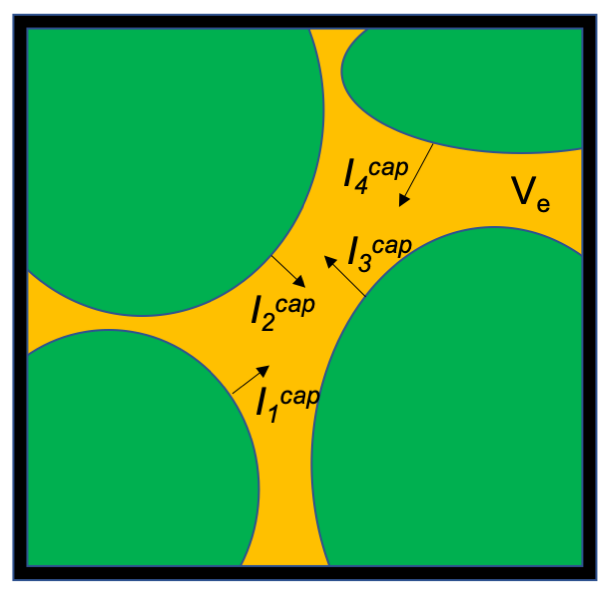
\includegraphics[width=0.5\textwidth]{Figures/Eldiff/KNP_Cap_illustration.png}
\end{center}
\caption{\textbf{Capacitive current sources}. Illustrated in terms of a finite volume of tissue, the capacitive current source density is the sum of capacitive currents entering the extracellular space from cells (green), divided by the fraction of the tissue volume that is extracellular (orange), i.e., $C_e^{cap} = \sum_k I_k^{cap}/V_e$. It can be interpreted as the accumulation of an extracellular charge density, which, since the bulk solution is assumed to be electroneutral, is associated exclusively by the charge accumulating at the exterior neural membranes.}
\label{Eldiff:fig:Ccap}
\end{figure}

Let us now look at the charge density, $\rho_e$ at the left hand side of eq. \ref{Eldiff:eq:chargecontinuity}. In general, $\rho_e$ could be composed of free charges in the extracellular bulk solution as well as charges bound to the outside of the neural membrane, i.e., we could have $\rho_e = \rho_e^{free} + \rho_e^{mem}$. However, as we have argued earlier, the bulk solution is very close to electroneutral, and if we assume perfect bulk electroneutrality ($\rho_e^{free} = 0$), we must have that $\rho_e=\rho_e^{mem}$. We can then combine eq. \ref{Eldiff:eq:chargecontinuity} with eq. \ref{Eldiff:eq:CSDdecomposed} to arrive at:

\begin{equation}
\nabla \cdot (\sigma_e\nabla\phi) = - C_e - F \nabla \cdot \left (\sum_k{z_k \tilde{D_k}{\bf \nabla} c_{k}} \right).
\label{Eldiff:eq:eldiffCSD2}
\end{equation}

Provided that the neuronal current sources $C_e$ and the extracellular ion concentrations $c_k$ are known at a given time, eq. \ref{Eldiff:eq:eldiffCSD2} can be solved for $\phi$. This solution for $\phi$ can be then be inserted into the Nernst-Planck system of equations (eq. \ref{Eldiff:eq:NP}), 
which can be solved for the temporal development of $c_k$ using some suitable numerical framework. It is the combination of eqns. \ref{Eldiff:eq:NP}) and \ref{Eldiff:eq:eldiffCSD2}, with $C_e$ as given in eq. \ref{Eldiff:eq:CSDdecomposed}, that defines the KNP scheme. 


\subsubsection{\blue{Comparison with volume conductor theory}}
Eq. \ref{Eldiff:eq:eldiffCSD2} is the electrodiffusive counterpart to eq. \ref{VC:eq:CSD2}, that we used as starting point in standard VC theory. For a more direct comparison, we can multiply eq.  \ref{Eldiff:eq:eldiffCSD2} with the extracellular volume fraction $\alpha$, and get:
\begin{equation}
\nabla \cdot (\sigma\nabla\phi) = - C - F\alpha \nabla \cdot \left (\sum_k{z_k \tilde{D_k}{\bf \nabla} c_{k}} \right).
\label{Eldiff:eq:eldiffCSD22}
\end{equation}
Comparing eq. \ref{Eldiff:eq:eldiffCSD22} and eq.  \ref{Eldiff:eq:eldiffCSD2}, we see that the difference is the last term in eq. \ref{Eldiff:eq:eldiffCSD22}, which is the diffusive contribution not accounted for in \ref{VC:eq:CSD2}. As eq. \ref{Eldiff:eq:eldiffCSD2} shows, also diffusive processes can contribute to the genesis of extracellular potentials, and if present, they could give rise to a non-zero $\phi$ even in the absence of neuronal sources ($C = 0$). Diffusive currents can thus be seen as an additional "source" for generating extracellular potentials \citep{Halnes2017}. 

As we showed in Chapter \ref{sec:VC}), eq. \ref{VC:eq:CSD2} (which is eq.  \ref{Eldiff:eq:eldiffCSD22} without the last term) allows us to derive an analytical expression for the electrical potential at all points in space once the $C$ is known. In comparison, the electrodiffusive counterpart (eq. \ref{Eldiff:eq:eldiffCSD22}) is more demanding to work with, as it requires finite element or finite difference solutions of the ion concentration dynamics in the three-dimensional extracellular space \cite{Solbra2018}. 


\subsubsection{\blue{Bi- and tri-domain models}}
\label{sec:Eldiff:domain}
\index{Domain models}
We should note that there exist a different category of tissue-scale electroneutral models, which have been inspired from by the bi-domain model by Eisenberg \citep{eisenberg1970}, which has previously been used to simulate cardiac tissue \citep{henriquez1993, sundnes2006, Mori2008}. 

In this category, the most advanced models for brain tissue are the tri-domain models, where three the domains represent (i) neurons, (ii) extracellular space, and (iii) a glial syncytium, i.e., a populations of gap-junction coupled glial cells \citep{OConnell2016, tuttle2019}. Simpler, related models include the bi-domain model for neurons and extracellular space \citep{Mori2015}, or 1D models of glial K$^+$ buffering, where only the glial and extracellular domain were included \cite{Gardner-Medwin1983, Chen2000, Halnes2013}.

The domain models do not model individual cells, but represents tissue as a (volume-averaged) continuum. All domains "exist" in parallel at each point in space, and are defined through a set of domain-specific variables (e.g., domain-voltage, domain-ion concentrations, domain-osmolarity, domain-volume fractions etc.). The domains interact locally through a set of (Hodgkin-Huxley type) membrane mechanisms, while spatial electrodiffusive transports may occur \textit{within} the domains. 

In the tri-domain models \citep{OConnell2016, tuttle2019}, intra-domain ion transport was assumed to occur in the glial and extracellular domain, but not the neural domain. The rationale behind that assumption was that a type of glial cells called astrocytes tend to be gap-junction coupled into a syncytium. In the syncytium, the intracellular space is more or less continuous in the same way that the extracellular space is continuous. Transport processes within the syncytium is then equivalent to extracellular transport in the sense that both take place in a continuous, tortous space. In contrast, neurons do not form synciti, and are "local" in the sense that no intracellular transport over distances occur within the neural domain (Fig.\ref{Eldiff:fig:domainmodel}). 

\begin{figure}[!ht]
\begin{center}
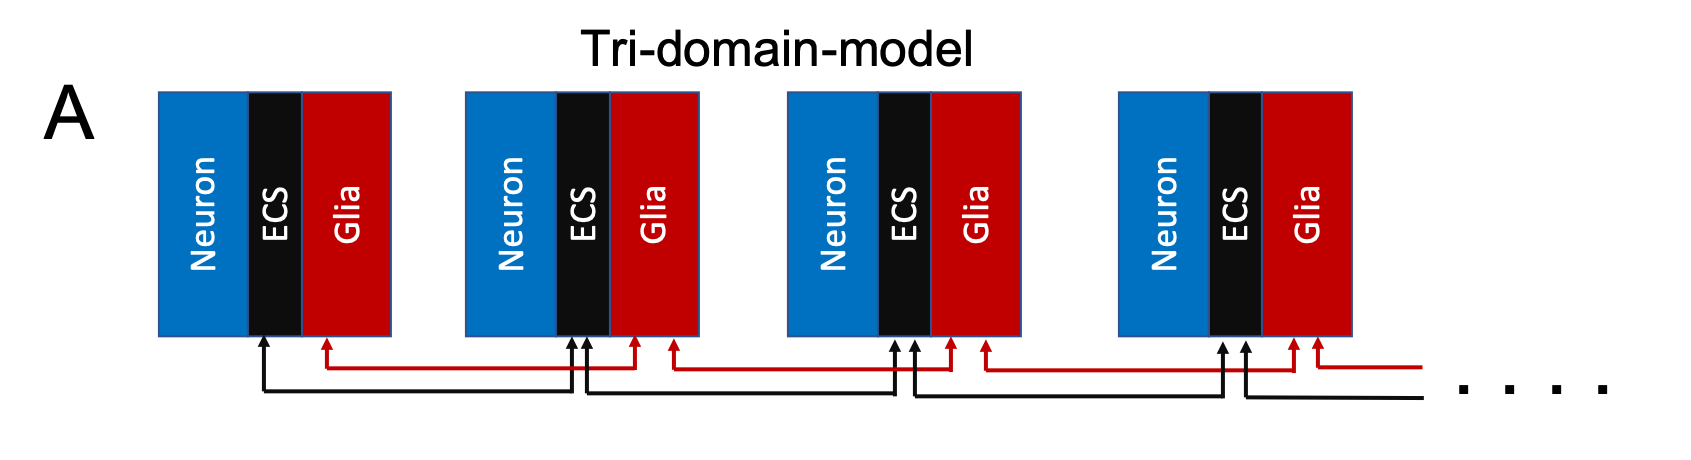
\includegraphics[width=0.8\textwidth]{Figures/Eldiff/Tridomain.png}
\end{center}
\caption{\textbf{Tri-domain model of brain tissue.} The domains represent neurons, extracellular space (ECS) and glial cells. The domains interact locally through transmembrane currents. Spatial ellectrodiffusion (arrows) occur within the ECS and glia domains, but not in within neuronal domain.The spatial dynamics can, in principle, occur in all directions (3D),but a 1D illustration was used in the figure. 
}
\label{Eldiff:fig:domainmodel}
\end{figure}

Domain models are suited to model brain dynamics taking place on large spatiotemporal scale, such as the wave of K$^+$ and the slow, DC-like diffusion potentials and glial buffering potentials that take place during the pathology of spreading depression \citep{Mori2015, OConnell2016, tuttle2019}. However, as these models treat all aspects of brain tissue as a homogeneous, coarse-grained continuum, they are not suited to model the faster fluctuations of extracellular potentials which are recorded in MUA, LFP and EEG, as these depend strongly on morphologies of neurons \citep{Einevoll2013}. 


\subsection{\blue{Do diffusion potentials matter?}}
\label{sec:Eldiff:estimates}
\index{Diffusion potential}
Due to the computational challenges they impose, it is tempting to make the assumption that diffusive currents contribute so little to the extracellular potential that we don't have to bother with them. This is what normally is being done, as most theoretical studies of extracellular potentials are based on standard VC theory. For most purposes, this is probably a good approximation, but its validity depends on one of the two following criteria being met:

\begin{enumerate}
\item C1: The magnitude of diffusive currents is much smaller than the magnitude of Ohmic drift currents.
\item C2: The frequency of diffusive currents is much lower than the frequency of the CSD and the Ohmic drift currents. 
\end{enumerate}

The first criterion is general and quite intuitive. If C1 holds, the last term in eq. \ref{Eldiff:eq:eldiffCSD2} becomes much smaller than the other two terms, and standard VC theory will give accurate predictions of $\phi$. As we shall see below, it is quite likely that C1 is violated under many physiological conditions. If so, the second criterion (C2) may still come to our rescue. In most experiments, extracellular potentials are recorded using electrode systems with a lower cut-off frequency of 0.1-1 Hz \citep{Einevoll2007}. As diffusive currents are proportional to concentration gradients, which generally vary at a much slower time scale than $\phi$, diffusive contributions to $\phi$ are often direct-current (DC) like, i.e., they vary very slowly with time, and if they vary slowly enough, they will not be picked up in recordings using standard electrode systems, but only in experiments using DC electrodes. The question regarding their contribution to standard measurements is then whether they vary slowly enough. 

In the two following subsections we shall explore when and to which degree the criteria C1-C2 are likely to be met under physiological conditions.

\subsubsection{\blue{Magnitude of diffusion potentials.}}
To make some crude estimation of the magnitude that we can expect diffusion potentials to have in neural tissue, we make the following simplifications of eq. \ref{Eldiff:eq:eldiffCSD2}): Firstly, diffusion potentials depend solely on extracellular concentration gradients, and not on the instantaneous activity of neurons. Let us therefore assume that $CSD = 0$, and consider the extracellular dynamics is governed by:
\begin{equation}
\nabla \cdot (\sigma_e\nabla\phi_d) = - \nabla \cdot \left (\sum_k{F z_k \tilde{D_k}{\bf \nabla} c_{k}} \right), 
\label{Eldiff:eq:eldiffCSD3}
\end{equation}
where we have denoted the potential $\phi_d$ since, in this case, it will exclusively be evoked by diffusion. Let us further consider a system with closed boundaries, so that no current can enter or leave the system. In that case, we may simply skip the first nabla, and take:
\begin{equation}
\sigma_e\nabla\phi_d = -\sum_k{F z_k \tilde{D_k}{\bf \nabla} c_{k}}, 
\label{Eldiff:eq:diffpot}
\end{equation}
Essentially, eq. \ref{Eldiff:eq:diffpot} states that the Ohmic drift current and diffusive current must cancel each others at each point in space, i.e., that if no current enters the system from the outside, no net current should be observed anywhere inside the system. The diffusion potential is thus the potential that we must have in the system for this to be the case. 

Finally, due to the linearity in eq. \ref{Eldiff:eq:diffpot}, the diffusion potential between two points in space is a direct function of the the ionic concentrations at these two points. Hence, it is sufficient for our task to consider a simple two-compartment system (like that in Fig. \ref{Eldiff:fig:diffpot}). For two-compartment systems, eq. \ref{Eldiff:eq:diffpot} further simplifies to:

\begin{equation}
\Delta \phi_d = \frac{F}{\bar{\sigma_e}} \sum_k{z_k \tilde{D}_k \Delta c_k}
\label{Eldiff:eq:diffpot2}
\end{equation}
where $\Delta c_k = c_{k}^{2} - c_{k}^{1}$ and $\Delta \phi_d = \phi_d^{2} - \phi_d^{1}$ denote the concentration and potential difference between compartments 1 and 2. Within each compartment, $\sigma_e$ can be determined from the ionic concentrations by use of eq. \ref{Eldiff:eq:sigma1}. However, since we for this problem need the conductivity experienced by an Ohmic current traveling between the two compartments, we have in eq. \ref{Eldiff:eq:diffpot2} used the average $\sigma_e$ of the two compartments:
\begin{equation}
\sigma_e = \frac{F}{2\psi}\sum_{k} \left(\tilde{D}_k z_{k}^2 c_{k}^{1} + \tilde{D}_k z_{k}^2 c_{k}^{2} \right).
\label{Eldiff:eq:sigma2}
\end{equation}

Based on eq. \ref{Eldiff:eq:diffpot2}, we make some estimates of the magnitude of the diffusion potential for some test examples.

\begin{itemize}

\item {\bf Diffusion potential under spreading depression:} The most extreme extracellular concentration shifts in the brain occur under the pathological condition called spreading depression, where the extracellular K$^+$ concentration can change by several tens of millomolars. In an an example from hippocampus, the K$^+$ concentration was about 30 mM higher at the bottom hippocampal layer than at the top hippocampal layer (Fig. 1a in \citep{Herreras1993}). In that experiment, only K$^+$ concentrations were recorded. However, we may give a crude estimate of the diffusion potential between the top and bottom of hippocampus by making some simple assumptions of the other ion concentrations: (i) We assume that the top layer of hippocampus remained at baseline concentrations. In the experiment, this seemed to be close to the case for $c_K$ \citep{Herreras1993}. In the top layer, we may therefore assume some rather typical baseline concentrations with $c_{Na} = 150$ mM, $c_{K} = 3$ mM and $c_{Cl} = 153$ mM. (ii) In the bottom layer, we assume that the $c_K$ was 30 mM above baseline, and that the increase in $c_K$ was compensated by an identical decrease in $c_{Na}$, so that electroneutrality was preserved. A plausible mechanism behind this would be that all concentration shifts were due to neuronal AP firing, i.e., neurons exchanging Na$^+$ for K$^+$. With these assumptions, we have $c_{Na} = 120$ mM, $c_{K} = 33$ mM and $c_{Cl} = 153$ mM in the bottom layer. Plugging the top layer and bottom layer concentrations into eq. \ref{Eldiff:eq:diffpot2}, we obtain a diffusion potential $\Delta \phi_d \sim 1$ mV across the hippocampal depth.

\item {\bf Diffusion potential in cortex during neuronal hyperactivity:} In several experimental papers, extracellular concentration shifts of selected ions have been recorded during induced neuronal hyperactivity and seizure activity \citep{kriv1975, nicholson1978, Dietzel1982, somjen1986, Dietzel1989}. The main focus of these works are typically on $c_K$, which is the most critical extracellular concentration due to its low baseline value. In these experiments, $c_K$ can typically change from a baseline value around 3 mM up to a ceiling level between 8-12 mM before the dynamics becomes pathological and is driven into spreading depression. Dietzel et al. estimated the concentration shifts in both $c_{K}$, $c_{Na}$ and $c_{Cl}$, and cased on a series of recordings, they estimated that the maximal diffusion potential that could be expected under their experimental condition was 0.4 mV \citep{Dietzel1989}.

\item{\bf Diffusion potential during normal activity:} It is difficult to find experimental data that allows us to estimate diffusion potentials in the brain under "normal" conditions, and the question as to whether concentration gradients are present in a given brain region probably depends on the processing state it is in. However, recordings from anesthetized cat cortex have shown that even during the resting state, $c_K$ may exhibit small-amplitude (0.5 mM) fluctuations \citep{MCCREERY1983}. In experiments recording the response in cortex to moderate (not seizure inducing) stimuli applied in the thalamus, cortical $c_K$ increases were found to have a depth profile, and vary by about 2 mM between different cortical layers \citep{Cordingley1978}. Thus, it seems likely that there should be some concentration gradients present in neural systems, and that e.g., a concentration difference of about 1 mM between the top and bottom of cortex or hippocampus would not be unlikely under normal processing. If we repeat the calculation from spreading depression, but assume that $c_{K}$ and $c_{Na}$ in the bottom layer were increased/decreased by 1 mM instead of 30 mM, we get a diffusion potential of about $33 \mu$V. This is of the same magnitude as potentials typically recorded in LFP recordings. 

\end{itemize}

Based on the crude estimates above, it is likely that many experimental conditions can contain diffusion potentials of the same magnitude as the potentials recorded in extracellular recordings, such as the LFP. 


\subsubsection{\red{GH: Frequency of diffusion potentials}}
\ghnote{Krevende kapittel. Sammenligne noen powerspectra her. Regne ut et par selv, ala Gratiy. Ser for meg at vi kanskje kjoerer eksemplene fra forrige delkap, og da lar konsentrasjonene falle til utjevining vha. diffusjon, samt et tilleggseksempel der vi lar dem falle eksponensielt med ulike tidskonstanter og bestemmer hvor raskt det maa gaa for at det skal fanges opp f.eks. ved 0.1 Hz. Da trenger vi paalitelige powerspectra fra eksperimentelle maalinger som vi kan sammenligne med. } 

Previous computational studies have predicted that effects of diffusion on extracellular potentials are not necessarily small, but tend to be very slow, meaning that they will only affect the very low-frequency components of $\phi$ \citep{Halnes2016, Halnes2017}. This is due to the diffusive current being a direct function of ion concentrations $c_k$, which on a large spatial scale typically vary on a much slower time scale (seconds-minutes) than the fluctuations in $\phi$ that we commonly are interested in (milliseconds-seconds). Furthermore, electrodes used to record $\phi$ typically have a lower cutoff frequency of 0.1-1Hz \citep{Einevoll2013}, which means that most of the tentative diffusive contribution will be filtered out from experimental recordings. It may therefore be a good approximation to neglect the diffusive term, except in the case of pathologically dramatic concentration variations.
